\documentclass{beamer}

\mode<presentation> {
}

\title[]{Bayesian Clinical Trials} 
\subtitle{Single Threshold Design} 
\date{} 

\usepackage{graphicx} 
\usepackage{booktabs} 
\usepackage{longtable} 
 \usepackage{hyperref}


\usepackage{color}
\usepackage{fancyvrb}

\definecolor{shadecolor}{gray}{0.95}

\DefineShortVerb[commandchars=\\\{\}]{\|}
\DefineVerbatimEnvironment{Highlighting}{Verbatim}{commandchars=\\\{\}}
\newenvironment{Shaded}{}{}
\newcommand{\KeywordTok}[1]{\textcolor[rgb]{0.00,0.44,0.13}{\textbf{{#1}}}}
\newcommand{\DataTypeTok}[1]{\textcolor[rgb]{0.56,0.13,0.00}{{#1}}}
\newcommand{\DecValTok}[1]{\textcolor[rgb]{0.25,0.63,0.44}{{#1}}}
\newcommand{\BaseNTok}[1]{\textcolor[rgb]{0.25,0.63,0.44}{{#1}}}
\newcommand{\FloatTok}[1]{\textcolor[rgb]{0.25,0.63,0.44}{{#1}}}
\newcommand{\CharTok}[1]{\textcolor[rgb]{0.25,0.44,0.63}{{#1}}}
\newcommand{\StringTok}[1]{\textcolor[rgb]{0.25,0.44,0.63}{{#1}}}
\newcommand{\CommentTok}[1]{\textcolor[rgb]{0.38,0.63,0.69}{\textit{{#1}}}}
\newcommand{\OtherTok}[1]{\textcolor[rgb]{0.00,0.44,0.13}{{#1}}}
\newcommand{\AlertTok}[1]{\textcolor[rgb]{1.00,0.00,0.00}{\textbf{{#1}}}}
\newcommand{\FunctionTok}[1]{\textcolor[rgb]{0.02,0.16,0.49}{{#1}}}
\newcommand{\RegionMarkerTok}[1]{{#1}}
\newcommand{\ErrorTok}[1]{\textcolor[rgb]{1.00,0.00,0.00}{\textbf{{#1}}}}
\newcommand{\NormalTok}[1]{{#1}}

\hypersetup{breaklinks=true, pdfborder={0 0 0}}
\setlength{\parindent}{0pt}
\setlength{\parskip}{6pt plus 2pt minus 1pt}
\setlength{\emergencystretch}{3em}  
\setcounter{secnumdepth}{0}
%\EndDefineVerbatimEnvironment{Highlighting}


\begin{document}



\begin{frame}
\titlepage % Print the title page as the first slide
\end{frame}


\begin{frame}{Phase II clinical trials}

\begin{itemize}
\itemsep1pt\parskip0pt\parsep0pt
\item
  \textbf{Features:} early trial in patients
\item
  \textbf{Purpose:}

  \begin{itemize}
  \itemsep1pt\parskip0pt\parsep0pt
  \item
    dose ranging
  \item
    adverse events
  \item
    pathophysiology
  \item
    limited efficacy data
  \end{itemize}
\item
  \textbf{Design:}

  \begin{itemize}
  \itemsep1pt\parskip0pt\parsep0pt
  \item
    single-stage
  \item
    multi-stage (Simon's optimal and minimax design)
  \end{itemize}
\end{itemize}

\end{frame}




\begin{frame}{Two-stage design}

\begin{itemize}
\itemsep1pt\parskip0pt\parsep0pt
\item
  A small group of patients are enrolled in the first stage
\item
  The enrollment of another group of patients in stage 2 is
  \emph{conditional} on the outcome of the first group

  \begin{itemize}
  \itemsep1pt\parskip0pt\parsep0pt
  \item
    activating the second stage depends on an adequate number of
    responses observed from the first stage
  \end{itemize}
\end{itemize}

 \textbf{Rationale:} to not enroll a large group of patients (as in
conventional one-stage designs) whether not sure if the new treatment is
effective

\end{frame}

\begin{frame}{Two-stage design}

\begin{itemize}
\item
  A phase II trial is an uncontrolle trial (tipically one-arm,
  open-label) to obtain an estimate of the degree of a new treatment
  (agent) effect
\item
  The aim is to see if the new agent has sufficient activity against a
  specific target (i.e, type of tumor, etc.) to warrant its further
  development

  \begin{itemize}
  \itemsep1pt\parskip0pt\parsep0pt
  \item
    to combine with other drugs in a phase III trial comparing survival
    results with a standard treatment
  \end{itemize}
\end{itemize}

\end{frame}

\begin{frame}{Single Threshold Design (STD)}

\begin{itemize}
\itemsep1pt\parskip0pt\parsep0pt
\item
  \(R_U\): target response
\item
  \(\pi_{prior}\): anticipated response rate
\item
  \(\lambda_1\) and \(\lambda_2\): threshold probabilities (at the
  interim stage and at the end of the trial) that the true response rate
  \(\pi\) exceeds \(R_U\)
\end{itemize}

Let the primary endpoint be a dichotomous variable \(X\) (e.g
\(X\sim Bin(n,\pi)\)):

-\(\pi\) represents the probability of success, for which a conjugate
prior \emph{Beta} distribution is chosen:
\(\pi\sim Beta(\alpha, \beta)\)

\end{frame}



\begin{frame}{Bayesian sample sizing as pre-posterior analysis}

\begin{itemize}
\itemsep1pt\parskip0pt\parsep0pt
\item
  \(R_U\): target response
\item
  \(\lambda\): minimum desired threshold probability that the true
  response rate \(\pi\) exceeds \(R_U\)
\end{itemize}

Suppose \(X\) is specified from the target response plus some small
value (e.g.~0.05): \[X=(R_U+0.05)\times n\]

The posterior probability \(P[(\pi\vert X,\alpha, \beta)>R_U]\) is computed:

\begin{itemize}
\itemsep1pt\parskip0pt\parsep0pt
\item
  if it exceeds \(\lambda \Longrightarrow n\) is the chosen sample size
\item
  if it does not exceeds \(\lambda \Longrightarrow\) the posterior
  calculation is repeated for \(n+1\) and continue until \(\lambda\) is
  exceeded.
\end{itemize}

\end{frame}

\begin{frame}{Two-stage design}

\begin{itemize}
\itemsep1pt\parskip0pt\parsep0pt
\item
  \(n\) patients are recruited to stage 1
\item
  possibily further \(N-n\) patients are recruited to stage 2
\end{itemize}

\textbf{Practical constraints:} There is often practical lower and upper
limits to the total study size N:

\begin{itemize}
\itemsep1pt\parskip0pt\parsep0pt
\item
  designs with stage 1 fewer than 5 patients are unlikely to be adopted
\item
  2 stage designs with N larger than 100 are unlikely to be adopted
\item
  typically total sample size \(N\) lies between 10 and 90
\end{itemize}

\end{frame}

\begin{frame}{Two-stage design}

Suppose \(X_1\) and \(X_2\) represent the hypothetical data that would
arise from the trial (they are specified from the target response
\(R_U\) plus some small value \(\epsilon_U\in(0,0.1)\) (e.g.~0.05)

We are searching for:

\begin{itemize}
\itemsep1pt\parskip0pt\parsep0pt
\item
  the smallest N for which \(P(\pi > R_U\vert X_1,X_2)>\lambda_2\)
\item
  at the same time, the smallest stage 1 sample size \(n\) such that:
  \(P(\pi > R_U\vert X_1)>\lambda_1\)
\end{itemize}

\end{frame}

\begin{frame}{Computational algorithms}

Tan\&Machin used a \(Beta(\alpha,\beta)\) vague prior distribution for
\(\pi\), where \[
\alpha = \pi_{prior} +1, \qquad \beta = (1-\pi_{prior})+1
\]

\begin{center}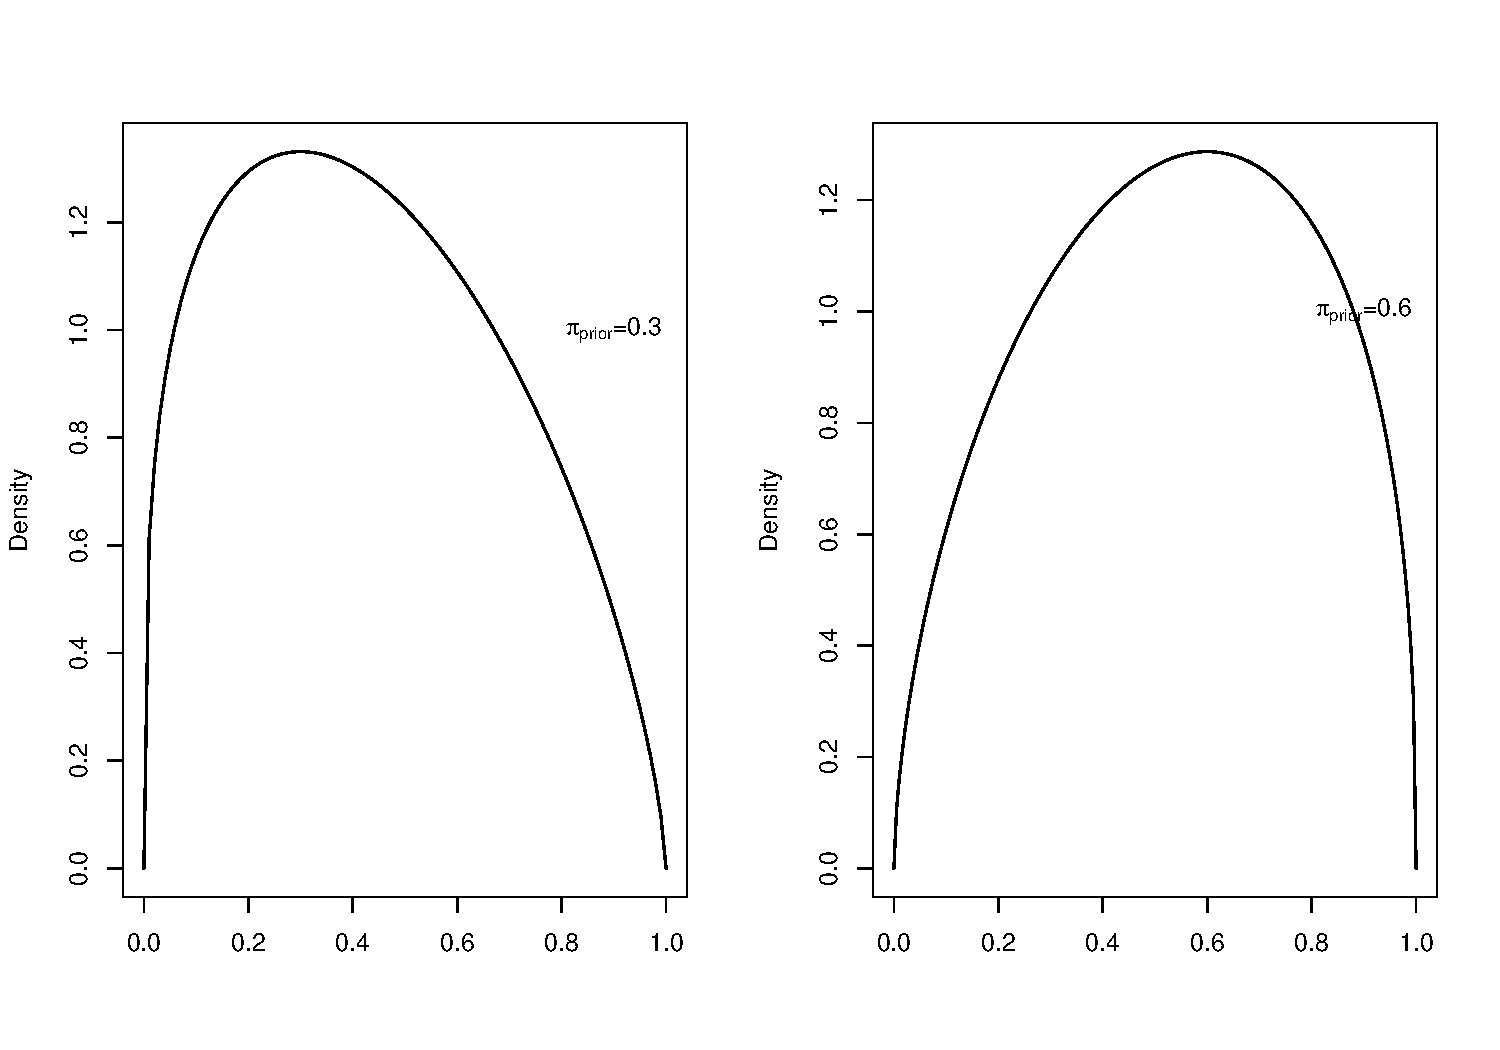
\includegraphics[scale=0.4]{06SingleThresholdDesign_files/figure-beamer/unnamed-chunk-1-1} \end{center}

\end{frame}

\begin{frame}{Computational algorithms}

\begin{itemize}
\item
  Specify \(R_U, \pi_{prior}, \lambda_1\) and \(\lambda_2\);
  \(\epsilon_U = 0.05\)
\item
  Set the overall number of successes as \(X=(R_U+\epsilon_U)\times N\),
  starting from \(N=10\)
  \(\Longrightarrow X \sim Binomial(N, R_U+\epsilon_U)\)
\item
  Set the prior \(\pi\sim Beta(\pi_{prior}+1; (1-\pi_{prior})+1)\)
\item
  Compute the posterior \[
  \pi\vert X_1,X_2,\alpha, \beta = Beta(\alpha';\beta') 
  \] where
\item
  \(\alpha' = \pi_{prior}+1+(R_U+\epsilon_U)\times N\)
\item
  \(\beta' = 1-\pi_{prior}+1+N-(R_U+\epsilon_U)\times N\)
\end{itemize}

\end{frame}

\begin{frame}{Priors}

Different ways to build prior distribution \(Beta(\alpha,\beta)\) for
\(\pi\):

\begin{itemize}
\itemsep1pt\parskip0pt\parsep0pt
\item
  Building priors solely on the prior parameters and interpreting
  \(\alpha + \beta\) as the total number of subjects (Gelman):

  \begin{itemize}
  \itemsep1pt\parskip0pt\parsep0pt
  \item
    \(\alpha\) successes and \(\beta\) failures
  \end{itemize}
\item
  Using 90th percent probability interval
  \(W_{90} = (5th, 95th)\)-percentiles and elicit information from
  investigators or past studies through the percentile approach
\end{itemize}

Informative and non-informative priors

\begin{itemize}
\itemsep1pt\parskip0pt\parsep0pt
\item
  \textbf{Informative priors} are narrow and reflect the knowledge of
  strong prior information
\item
  \textbf{Non-informative priors} are flat and reflect little prior
  information
\end{itemize}

\end{frame}

\begin{frame}{Prior elicitation}

Two steps for eliciting a-priori distribution

\begin{enumerate}
\def\labelenumi{\arabic{enumi}.}
\itemsep1pt\parskip0pt\parsep0pt
\item
  eliciting the center value by asking the clinician ``what is the most
  likely response reate you expect to occur?''

  \begin{itemize}
  \itemsep1pt\parskip0pt\parsep0pt
  \item
    finding out whether the response is the mean, median or the mode
  \end{itemize}
\item
  assessing the uncertainty in the ``most likely response rate''

  \begin{itemize}
  \itemsep1pt\parskip0pt\parsep0pt
  \item
    elicitation of \(W_{90}\) is easy for clinicians who think in terms
    of percentiles
  \item
    \(W_{90}\) can be elicited by asking clinicians how uncertain they
    are regarding their center value
  \item
    for mode answer, the question can be posed as ``prior sample size''
    (increasing or decreasing \(\alpha + \beta\))
  \end{itemize}
\end{enumerate}

\end{frame}

\begin{frame}{How to build priors}

\begin{enumerate}
\def\labelenumi{\arabic{enumi}.}
\item
  \textbf{mode (non-informative):}

  \begin{itemize}
  \itemsep1pt\parskip0pt\parsep0pt
  \item
    it has prior parameters \(\alpha = \pi_{prior}+1\) and
    \(\beta = 1-\pi_{prior}+1\)
  \item
    it has the interpretation of a mode and a prior sample size of
    \(\alpha+\beta=3\)
  \end{itemize}
\item
  \textbf{mode (informative):}

  \begin{itemize}
  \itemsep1pt\parskip0pt\parsep0pt
  \item
    it has prior parameters
    \(\alpha = \pi_{prior}+1+n_{prior}\pi_{prior}\) and
    \(\beta = 1-\pi_{prior}+1+n_{prior}(1-\pi_{prior})\)
  \item
    it has the interpretation of a mode and a prior sample size of
    \(\alpha+\beta=n_{prior}+3\)
  \end{itemize}
\end{enumerate}

\end{frame}



\begin{frame}{How to build priors}

\begin{enumerate}
\def\labelenumi{\arabic{enumi}.}
\setcounter{enumi}{2}
\item
  \textbf{median (informative):}

  \begin{itemize}
  \itemsep1pt\parskip0pt\parsep0pt
  \item
    we elicit \(\pi_{prior}\) assuming it is the \emph{median} and we
    elicit also \(W_{90}\)
  \item
    this requires solving the system:
  \end{itemize}
\end{enumerate}

$$
F(\pi_{prior}\vert \alpha\beta) =0.5 
$$
$$
F^{-1}(0.95\vert \alpha\beta) -F^{-1}(0.05\vert \alpha\beta) = W_{90} 
$$


\begin{enumerate}
\def\labelenumi{\arabic{enumi}.}
\setcounter{enumi}{3}
\item
  \textbf{mean (informative):}

  \begin{itemize}
  \itemsep1pt\parskip0pt\parsep0pt
  \item
    we elicit \(\pi_{prior}\) assuming it is the \emph{mean} and we
    elicit also \(W_{90}\)
  \item
    this requires solving the system:
  \end{itemize}
\end{enumerate}

$$
E(y)=\pi_{prior} 
$$
$$
F^{-1}(0.95\vert \alpha\beta) -F^{-1}(0.05\vert \alpha\beta) = W_{90} 
$$

\end{frame}



\begin{frame}[fragile]{Sample size calculation}

\begin{Shaded}
\begin{Highlighting}[]
\KeywordTok{source}\NormalTok{(}\StringTok{'R/singleThresholdDesign.R'}\NormalTok{)}
\KeywordTok{source}\NormalTok{(}\StringTok{'R/informativePriors.R'}\NormalTok{)}
\end{Highlighting}
\end{Shaded}

\begin{itemize}
\item
  sample size calcultion using the \textbf{non-informative mode} prior:
\item
  \(R_U=0.2\), \(\pi_{prior}=R_U+0.05\) and \(\lambda=0.8\)
\end{itemize}


\begin{Shaded}
\begin{Highlighting}[]
\KeywordTok{stage2}\NormalTok{(}\DataTypeTok{ru =} \FloatTok{0.2}\NormalTok{, }\DataTypeTok{pi =} \FloatTok{0.2} \NormalTok{+}\StringTok{ }\FloatTok{0.05}\NormalTok{, }\DataTypeTok{lambda =} \FloatTok{0.8}\NormalTok{)}
\end{Highlighting}
\end{Shaded}

\begin{verbatim}
## $N
## [1] 32
## 
## $posterior
## [1] 0.8023008
\end{verbatim}

\end{frame}






\begin{frame}[fragile]{Sample size calculation}

\begin{itemize}
\item
  Sample size calculation using the \textbf{informative mode} prior with
  \(n_{prior}=10\):
\item
  \(R_U=0.2\), \(\pi_{prior}=R_U+0.05\), \(W_{90}=0.3\) and
  \(\lambda=0.8\)
\end{itemize}

\begin{Shaded}
\begin{Highlighting}[]
\KeywordTok{pparameter}\NormalTok{(}\DataTypeTok{pi=}\FloatTok{0.2+0.05}\NormalTok{, }\DataTypeTok{w90=}\FloatTok{0.3}\NormalTok{, }\DataTypeTok{prior.method=}\StringTok{'mode-informative'}\NormalTok{)}
\end{Highlighting}
\end{Shaded}

\begin{verbatim}
## $alpha
## [1] 3.75
## 
## $beta
## [1] 9.25
\end{verbatim}

\begin{Shaded}
\begin{Highlighting}[]
\KeywordTok{stage2}\NormalTok{(}\DataTypeTok{ru=}\FloatTok{0.2}\NormalTok{, }\DataTypeTok{pi=}\FloatTok{0.2+0.05}\NormalTok{, }\DataTypeTok{lambda=}\FloatTok{0.8}\NormalTok{, }\DataTypeTok{alpha =} \FloatTok{3.75}\NormalTok{, }\DataTypeTok{beta =} \FloatTok{9.25}\NormalTok{)}
\end{Highlighting}
\end{Shaded}

\begin{verbatim}
## $N
## [1] 22
## 
## $posterior
## [1] 0.8023008
\end{verbatim}

\end{frame}




\begin{frame}[fragile]{Sample size calculation}

\begin{itemize}
\item
  Sample size calculation using the \textbf{informative median} prior:
\item
  \(R_U=0.2\), \(\pi_{prior}=R_U+0.05\), \(W_{90}=0.3\) and
  \(\lambda=0.8\)
\end{itemize}

\begin{Shaded}
\begin{Highlighting}[]
\KeywordTok{pparameter}\NormalTok{(}\DataTypeTok{pi=}\FloatTok{0.2+0.05}\NormalTok{, }\DataTypeTok{w90=}\FloatTok{0.3}\NormalTok{, }\DataTypeTok{prior.method=}\StringTok{'median-informative'}\NormalTok{)}
\end{Highlighting}
\end{Shaded}

\begin{verbatim}
## $alpha
## [1] 5.613544
## 
## $beta
## [1] 16.1849
\end{verbatim}

\begin{Shaded}
\begin{Highlighting}[]
\KeywordTok{stage2}\NormalTok{(}\DataTypeTok{ru=}\FloatTok{0.2}\NormalTok{, }\DataTypeTok{pi=}\FloatTok{0.2+0.05}\NormalTok{, }\DataTypeTok{lambda=}\FloatTok{0.8}\NormalTok{, }\DataTypeTok{alpha =} \FloatTok{5.61}\NormalTok{, }\DataTypeTok{beta =} \FloatTok{16.19}\NormalTok{)}
\end{Highlighting}
\end{Shaded}

\begin{verbatim}
## $N
## [1] 27
## 
## $posterior
## [1] 0.8005037
\end{verbatim}

\end{frame}



\begin{frame}[fragile]{Sample size calculation}

\begin{itemize}
\item
  Sample size calculation using the \textbf{informative mean} prior:
\item
  \(R_U=0.2\), \(\pi_{prior}=R_U+0.05\), \(W_{90}=0.3\) and
  \(\lambda=0.8\)
\end{itemize}

\begin{Shaded}
\begin{Highlighting}[]
\KeywordTok{pparameter}\NormalTok{(}\DataTypeTok{pi=}\FloatTok{0.2+0.05}\NormalTok{, }\DataTypeTok{w90=}\FloatTok{0.3}\NormalTok{, }\DataTypeTok{prior.method=}\StringTok{'mean-informative'}\NormalTok{)}
\end{Highlighting}
\end{Shaded}

\begin{verbatim}
## $alpha
## [1] 5.331685
## 
## $beta
## [1] 15.99505
\end{verbatim}

\begin{Shaded}
\begin{Highlighting}[]
\KeywordTok{stage2}\NormalTok{(}\DataTypeTok{ru=}\FloatTok{0.2}\NormalTok{, }\DataTypeTok{pi=}\FloatTok{0.2+0.05}\NormalTok{, }\DataTypeTok{lambda=}\FloatTok{0.8}\NormalTok{, }\DataTypeTok{alpha =} \FloatTok{5.33}\NormalTok{, }\DataTypeTok{beta =} \DecValTok{16}\NormalTok{)}
\end{Highlighting}
\end{Shaded}

\begin{verbatim}
## $N
## [1] 34
## 
## $posterior
## [1] 0.80136
\end{verbatim}

\end{frame}



\begin{frame}{Pessimistic and optimistic sample size calculations}

Using the routines provided, try to find the sample size for different
values of \(R_U\) according to these definitions of:

\begin{itemize}
\itemsep1pt\parskip0pt\parsep0pt
\item
  \textbf{very optimistic prior}: \(\pi_{prior} = R_U + 0.05\)
\item
  \textbf{optimistic prior}: \(\pi_{prior} = R_U\)
\item
  \textbf{pessimistic prior}: \(\pi_{prior} = R_U -0.2\)
\end{itemize}

\end{frame}

\begin{frame}[fragile]{Fill in the table}

\begin{longtable}[c]{@{}lllll@{}}
\toprule
\begin{minipage}[b]{0.09\columnwidth}\raggedright\strut
\(R_U\)
\strut\end{minipage} &
\begin{minipage}[b]{0.34\columnwidth}\raggedright\strut
Prior Type
\strut\end{minipage} &
\begin{minipage}[b]{0.17\columnwidth}\raggedright\strut
Very Optimistic
\strut\end{minipage} &
\begin{minipage}[b]{0.12\columnwidth}\raggedright\strut
Optimistic
\strut\end{minipage} &
\begin{minipage}[b]{0.13\columnwidth}\raggedright\strut
Pessimistic
\strut\end{minipage}\tabularnewline
\midrule
\endhead
\begin{minipage}[t]{0.09\columnwidth}\raggedright\strut
0.40
\strut\end{minipage} &
\begin{minipage}[t]{0.34\columnwidth}\raggedright\strut
\begin{itemize}
\itemsep1pt\parskip0pt\parsep0pt
\item
  non informative mode
\item
  informative mode \(n_{prior=10}\)
\item
  informative median
\item
  informative mean
\end{itemize}
\strut\end{minipage} &
\begin{minipage}[t]{0.17\columnwidth}\raggedright\strut
\begin{itemize}
\item
\item
\item
\item
\end{itemize}
\strut\end{minipage} &
\begin{minipage}[t]{0.12\columnwidth}\raggedright\strut
\strut\end{minipage} &
\begin{minipage}[t]{0.13\columnwidth}\raggedright\strut
\strut\end{minipage}\tabularnewline
\begin{minipage}[t]{0.09\columnwidth}\raggedright\strut
0.70
\strut\end{minipage} &
\begin{minipage}[t]{0.34\columnwidth}\raggedright\strut
\begin{itemize}
\itemsep1pt\parskip0pt\parsep0pt
\item
  non informative mode
\item
  informative mode \(n_{prior=10}\)
\item
  informative median
\item
  informative mean
\end{itemize}
\strut\end{minipage} &
\begin{minipage}[t]{0.17\columnwidth}\raggedright\strut
\begin{itemize}
\item
\item
\item
\item
\end{itemize}
\strut\end{minipage} &
\begin{minipage}[t]{0.12\columnwidth}\raggedright\strut
\strut\end{minipage} &
\begin{minipage}[t]{0.13\columnwidth}\raggedright\strut
\strut\end{minipage}\tabularnewline
\bottomrule
\end{longtable}

\end{frame}





\begin{frame}{Sample size versus \(W_{90}\)}

\begin{itemize}
\itemsep1pt\parskip0pt\parsep0pt
\item
  \(R_U=0.2\), \(\pi_{prior}=R_U\)
\end{itemize}

\end{frame}

\begin{frame}{Sample size versus \(W_{90}\)}

Plot the relationship between \(W_{90}\) and sample size \(n\) for
\(R_U=0.6\) for

\begin{itemize}
\itemsep1pt\parskip0pt\parsep0pt
\item
  \textbf{very optimistic prior}: \(\pi_{prior} = R_U + 0.05\)
\item
  \textbf{optimistic prior}: \(\pi_{prior} = R_U\)
\item
  \textbf{pessimistic prior}: \(\pi_{prior} = R_U -0.2\)
\end{itemize}

\end{frame}

\begin{frame}[fragile]{R code}

\begin{Shaded}
\begin{Highlighting}[]
\NormalTok{w90=}\KeywordTok{seq}\NormalTok{(}\DataTypeTok{from=}\FloatTok{0.3}\NormalTok{, }\DataTypeTok{to=}\FloatTok{0.8}\NormalTok{, }\DataTypeTok{length.out =} \DecValTok{25}\NormalTok{)}
\NormalTok{ru=}\FloatTok{0.2}\NormalTok{; pi=ru; lambda=}\FloatTok{0.8}
\NormalTok{n.ni=}\OtherTok{NULL}\NormalTok{; n.med=}\OtherTok{NULL}\NormalTok{; n.mea=}\OtherTok{NULL}

\NormalTok{for(i in }\DecValTok{1}\NormalTok{:}\KeywordTok{length}\NormalTok{(w90))\{}
  \NormalTok{n.ni[i] =}\StringTok{ }\KeywordTok{stage2}\NormalTok{(}\DataTypeTok{ru=}\NormalTok{ru, }\DataTypeTok{pi=}\NormalTok{pi, }\DataTypeTok{lambda =} \NormalTok{lambda)}
  \NormalTok{param =}\StringTok{ }\KeywordTok{pparameter}\NormalTok{(}\DataTypeTok{pi=}\NormalTok{pi, }\DataTypeTok{w90=}\NormalTok{w90[i], }\DataTypeTok{prior.method=}\StringTok{'median-informative'}\NormalTok{)}
  \NormalTok{n.med[i] =}\StringTok{ }\KeywordTok{stage2}\NormalTok{(}\DataTypeTok{ru=}\NormalTok{ru, }\DataTypeTok{pi=}\NormalTok{pi, }\DataTypeTok{lambda =} \NormalTok{lambda, }\DataTypeTok{alpha =} \NormalTok{param$alpha, }\DataTypeTok{beta =} \NormalTok{param$beta)}
  \NormalTok{param =}\StringTok{ }\KeywordTok{pparameter}\NormalTok{(}\DataTypeTok{pi=}\NormalTok{pi, }\DataTypeTok{w90=}\NormalTok{w90[i], }\DataTypeTok{prior.method=}\StringTok{'mean-informative'}\NormalTok{)}
  \NormalTok{n.mea[i] =}\StringTok{ }\KeywordTok{stage2}\NormalTok{(}\DataTypeTok{ru=}\NormalTok{ru, }\DataTypeTok{pi=}\NormalTok{pi, }\DataTypeTok{lambda =} \NormalTok{lambda, }\DataTypeTok{alpha =} \NormalTok{param$alpha, }\DataTypeTok{beta =} \NormalTok{param$beta)}
\NormalTok{\}}
\KeywordTok{plot}\NormalTok{(w90, }\KeywordTok{unlist}\NormalTok{(n.ni), }\DataTypeTok{lty=}\StringTok{'solid'}\NormalTok{, }\DataTypeTok{xlim=}\KeywordTok{c}\NormalTok{(}\FloatTok{0.2}\NormalTok{,}\FloatTok{0.9}\NormalTok{),}\DataTypeTok{ylim=}\KeywordTok{c}\NormalTok{(}\DecValTok{20}\NormalTok{,}\DecValTok{80}\NormalTok{), }\DataTypeTok{ylab=}\StringTok{'n'}\NormalTok{)}
\KeywordTok{lines}\NormalTok{(w90, }\KeywordTok{unlist}\NormalTok{(n.med), }\DataTypeTok{lty=}\StringTok{'dotted'}\NormalTok{)}
\KeywordTok{lines}\NormalTok{(w90, }\KeywordTok{unlist}\NormalTok{(n.mea), }\DataTypeTok{lty=}\StringTok{'longdash'}\NormalTok{)}
\KeywordTok{legend}\NormalTok{(}\StringTok{'topright'}\NormalTok{, }\DataTypeTok{lty=}\KeywordTok{c}\NormalTok{(}\StringTok{'solid'}\NormalTok{,}\StringTok{'dotted'}\NormalTok{,}\StringTok{'longdash'}\NormalTok{), }
       \DataTypeTok{legend=}\KeywordTok{c}\NormalTok{(}\StringTok{'non-informative'}\NormalTok{,}\StringTok{'median'}\NormalTok{,}\StringTok{'mean'}\NormalTok{))}
\end{Highlighting}
\end{Shaded}

\end{frame}




\begin{frame}[fragile]{Case Study}

\begin{itemize}
\itemsep1pt\parskip0pt\parsep0pt
\item
  Phase II clinical trial to assess the response to gemcitabile plus
  docetaxel among patients with leiomyosarcome (LMS)
\end{itemize}

\end{frame}



\begin{frame}{Problem statistical setup}

\begin{itemize}
\itemsep1pt\parskip0pt\parsep0pt
\item
  \textbf{endpoint:} (binary) tumor response: yes/no (Response Criteria)
\item
  \textbf{null hypothesis:} \(H_0: \pi = \pi_0\)

  \begin{itemize}
  \itemsep1pt\parskip0pt\parsep0pt
  \item
    \(\pi\) is the true response (proportion of patients whose tumors
    shrink by at least 30\%)
  \item
    \(\pi_0\) is a predetermined undesirable level (pu)
  \end{itemize}
\item
  \textbf{alternative hypothesis:} \(H_A: \pi = \pi_A\)

  \begin{itemize}
  \itemsep1pt\parskip0pt\parsep0pt
  \item
    \(\pi_A\) is a desirable response rate (pa) \_ \textbf{Type I and
    type II errors:} \(\alpha\) and \(\beta\)
  \end{itemize}
\item
  \textbf{basis for decision:} minimize the number of patients treated
  in the trial if \(H_0\) is true
\end{itemize}

\end{frame}

\begin{frame}{The two stage design}

\begin{itemize}
\itemsep1pt\parskip0pt\parsep0pt
\item
  enroll \(n_1\) patients at stage 1:

  \begin{itemize}
  \itemsep1pt\parskip0pt\parsep0pt
  \item
    the trial is stopped if \(r_1\) or fewer responses are observed
  \item
    otherwise goes on to the second stage
  \end{itemize}
\item
  enross \(n_2\) patients at stage 2:

  \begin{itemize}
  \itemsep1pt\parskip0pt\parsep0pt
  \item
    the trial is not recommended for further development if a total of
    \(r (r > r_1)\) or fewer responses are observed at both stages
  \end{itemize}
\end{itemize}

\end{frame}

\begin{frame}{Probability of early termination and expected sample size}

PET: the probability to observe \(r_1\) or fewer responses at the first
stage

\[
PET(\pi) = P(R_1\leq r_1\vert n_1, \pi)
\] where P is the cumulative Binomial probability.

EN: expected sample size \[
EN(\pi)= n_1 + (1-PET(\pi))\times n_2
\]

\end{frame}



\begin{frame}{Probability of not recommending (PNR)}

The drug is not remmended if the trial is terminated early (i.e.~fewer
than \(r_1\) responses are observed at the first stage) or fewer than
\(r = r_1 + r_2\) are observed at the end of both stages

\[
PNR(\pi) = P(R_1\leq r_1\vert n_1, \pi) + \sum_{x=r_1+1}^{\min(n_1,r)} Binom(x\vert n_1,\pi)\times P(R\leq r-x\vert n_1, \pi)
\]

\end{frame}

\begin{frame}{Two types of errors}

\begin{itemize}
\itemsep1pt\parskip0pt\parsep0pt
\item
  type I error: \(\alpha = 1- PNR(\pi_0)\)
\item
  type II error: \(\beta = 1- PNR(\pi_A)\)
\end{itemize}

\end{frame}

\begin{frame}{Simon's approach}

\begin{itemize}
\itemsep1pt\parskip0pt\parsep0pt
\item
  Specify the parameters \(\pi_0\), \(\pi_A\), \(\alpha\) and \(\beta\)
\item
  Determine the two stage design that satisfies the errors probabilities
  \(\alpha\) and \(\beta\) and minimizes the expected sample size when
  the response probability is \(\pi_0\) (optimal design)
\item
  Determine the two stage design that satisfies the errors probabilities
  \(\alpha\) and \(\beta\) and minimizes the maximum sample size when
  the response probability is \(\pi_0\) (minimax design)
\end{itemize}

\end{frame}

\begin{frame}[fragile]{Sample size according to Simon two-stage design}

\begin{Shaded}
\begin{Highlighting}[]
\KeywordTok{library}\NormalTok{(clinfun)}
\end{Highlighting}
\end{Shaded}

\begin{verbatim}
## Warning: package 'clinfun' was built under R version 3.2.2
\end{verbatim}

\begin{Shaded}
\begin{Highlighting}[]
\KeywordTok{ph2simon}\NormalTok{(}\DataTypeTok{pu=}\FloatTok{0.05}\NormalTok{, }\DataTypeTok{pa=}\FloatTok{0.15}\NormalTok{, }\DataTypeTok{ep1=}\FloatTok{0.05}\NormalTok{, }\DataTypeTok{ep2=}\FloatTok{0.3}\NormalTok{)}
\end{Highlighting}
\end{Shaded}

\begin{verbatim}
## 
##  Simon 2-stage Phase II design 
## 
## Unacceptable response rate:  0.05 
## Desirable response rate:  0.15 
## Error rates: alpha =  0.05 ; beta =  0.3 
## 
##         r1 n1 r  n EN(p0) PET(p0)
## Optimal  1 19 4 43  24.89  0.7547
## Minimax  0 17 4 39  29.80  0.4181
\end{verbatim}

\end{frame}

\begin{frame}[fragile]{Sample size according to Simon two-stage design}

\begin{Shaded}
\begin{Highlighting}[]
\KeywordTok{library}\NormalTok{(clinfun)}

\KeywordTok{plot}\NormalTok{(}\KeywordTok{ph2simon}\NormalTok{(}\DataTypeTok{pu=}\FloatTok{0.05}\NormalTok{, }\DataTypeTok{pa=}\FloatTok{0.15}\NormalTok{, }\DataTypeTok{ep1=}\FloatTok{0.05}\NormalTok{, }\DataTypeTok{ep2=}\FloatTok{0.3}\NormalTok{))}
\end{Highlighting}
\end{Shaded}

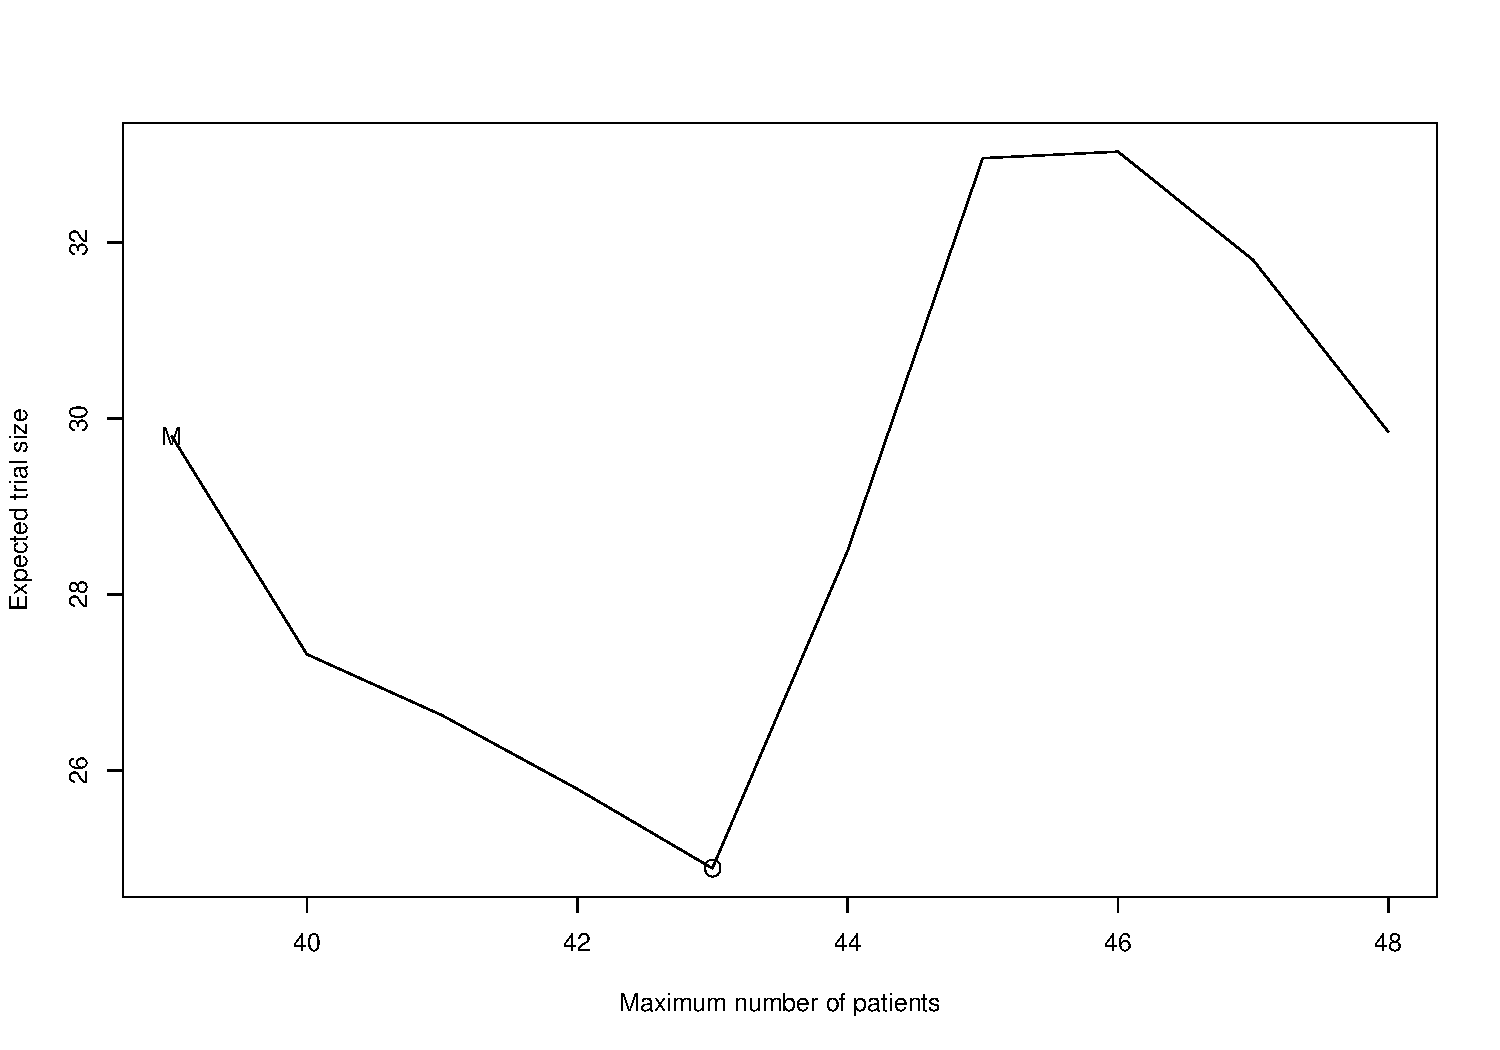
\includegraphics[scale=0.4]{06SingleThresholdDesign_files/figure-beamer/unnamed-chunk-9-1.pdf}

\end{frame}

\begin{frame}{STD Design}

Try to find the number of patients enrolled if a STD was adopted using
for comparatibe purposes:

\begin{itemize}
\itemsep1pt\parskip0pt\parsep0pt
\item
  a non informative very optimistic prior (\(\pi_{prior}=R_U+0.05\) )
\item
  an informative mode prior (\(n_{prior}=10\))
\item
  the median and mean ifnormative priors with \(W_{90}=0.3\)
\end{itemize}

\end{frame}

\begin{frame}[fragile]{R code}

\begin{Shaded}
\begin{Highlighting}[]
\KeywordTok{stage2}\NormalTok{(}\DataTypeTok{ru=}\FloatTok{0.15}\NormalTok{, }\DataTypeTok{pi=}\FloatTok{0.2}\NormalTok{, }\DataTypeTok{lambda=}\FloatTok{0.8}\NormalTok{)}

\KeywordTok{pparameter}\NormalTok{(}\DataTypeTok{pi=}\FloatTok{0.2}\NormalTok{, }\DataTypeTok{w90=}\FloatTok{0.3}\NormalTok{, }\DataTypeTok{prior.method=}\StringTok{'mode-informative'}\NormalTok{)}
\KeywordTok{stage2}\NormalTok{(}\DataTypeTok{ru=}\FloatTok{0.15}\NormalTok{, }\DataTypeTok{pi=}\FloatTok{0.2}\NormalTok{, }\DataTypeTok{lambda=}\FloatTok{0.8}\NormalTok{, }\DataTypeTok{alpha =} \FloatTok{3.2}\NormalTok{, }\DataTypeTok{beta =} \FloatTok{9.8}\NormalTok{)}

\KeywordTok{pparameter}\NormalTok{(}\DataTypeTok{pi=}\FloatTok{0.2}\NormalTok{, }\DataTypeTok{w90=}\FloatTok{0.3}\NormalTok{, }\DataTypeTok{prior.method=}\StringTok{'median-informative'}\NormalTok{)}
\KeywordTok{stage2}\NormalTok{(}\DataTypeTok{ru=}\FloatTok{0.15}\NormalTok{, }\DataTypeTok{pi=}\FloatTok{0.2}\NormalTok{, }\DataTypeTok{lambda=}\FloatTok{0.8}\NormalTok{, }\DataTypeTok{alpha =} \FloatTok{3.91}\NormalTok{, }\DataTypeTok{beta =} \FloatTok{14.68}\NormalTok{)}

\KeywordTok{pparameter}\NormalTok{(}\DataTypeTok{pi=}\FloatTok{0.2}\NormalTok{, }\DataTypeTok{w90=}\FloatTok{0.3}\NormalTok{, }\DataTypeTok{prior.method=}\StringTok{'mean-informative'}\NormalTok{)}
\KeywordTok{stage2}\NormalTok{(}\DataTypeTok{ru=}\FloatTok{0.15}\NormalTok{, }\DataTypeTok{pi=}\FloatTok{0.2}\NormalTok{, }\DataTypeTok{lambda=}\FloatTok{0.9}\NormalTok{, }\DataTypeTok{alpha =} \FloatTok{3.55}\NormalTok{, }\DataTypeTok{beta =} \FloatTok{14.23}\NormalTok{)}
\end{Highlighting}
\end{Shaded}

\end{frame}



\end{document}